\documentclass[12pt]{article}

\usepackage{fullpage}
\usepackage{graphicx, rotating, booktabs} 
\usepackage{times} 
\usepackage{natbib} 
\usepackage{indentfirst} 
\usepackage{setspace}
\usepackage{grffile} 
\usepackage{hyperref}
\usepackage{adjustbox}
\setcitestyle{aysep{}}


\singlespace
\title{\textbf{Appendix: Alliance Participation, Treaty Depth, and Military Spending}}
%\author{Joshua Alley}
\date{}

\bibliographystyle{apsr}

\begin{document}

\maketitle 

\doublespace 

This online appendix provides more detail about the multilevel model and checks the results. I also briefly describe a single-level test of the depth hypothesis and assess other measures of alliance treaty depth. 


\section{Control Variables} 


In the state-level regression, I adjust for several correlates of alliance participation and military spending. 
State-level covariates include GDP growth \citep{Boltetal2018} regime type, international war \citep{Reiteretal2016}, civil war participation \citep{SarkeesWayman2010}, annual MIDs \citep{Gibleretal2016}, rival military spending \citep{ThompsonDreyer2012} and a dummy for Cold War years.
Conflict participation, alliances, and military spending are all correlated \citep{SeneseVasquez2008}.
I include growth in GDP instead of levels because GDP levels are non-stationary and economic growth shapes the opportunity costs of military spending \citep{Kimball2010, Zielinskietal2017}.  

 
Other alliance level variables are correlates of treaty design and military spending, including the number of members and share of democracies in a treaty at time of formation \citep{Chibaetal2015}. 
I control for issue linkages by creating a dummy indicator of whether the alliance promises any kind of economic cooperation \citep{Poast2013, LongLeeds2006}. 
As an indicator of hierarchical security relationships, I include a count of foreign policy concessions in the alliance. 
I also mark the presence of unconditional military support using a dummy variable I constructed using existing indicators of conditional support in the ATOP data. 
I adjust for superpower membership--- whether the United States or Soviet Union participated in a treaty during the Cold War. 
Two dummy indicators of wartime alliances and asymmetric obligations \citep{Leedsetal2002} complete the alliance-level regression specification. 
Though I discuss these variables as controls, many of them are theoretically interesting in their own right. 


\section{Priors}

\autoref{tab:priors} summarizes the prior distributions in the multilevel model. 
All priors are weakly informative relative to the scale of the data. 
$\nu$ is the degrees of freedom for the t-distribution, and the gamma prior is the recommended default prior for STAN. 

\begin{table} % Create a table of priors.
\begin{center}
\begin{tabular}{c} 
$ p(\alpha) \sim N(0, 1)$  \\
$ p(\sigma) \sim \mbox{half-}N(0, 1) $ \\
$ p(\alpha^{yr}) \sim N(0, \sigma^{yr}) $ \\ 
$ p(\sigma^{yr}) \sim N(0, 1) $ \\
$ p(\alpha^{st}) \sim N(0, \sigma^{st}) $ \\ 
$ p(\sigma^{st}) \sim \mbox{half-}N(0, .5) $ \\ 
$ p(\sigma^{all}) \sim \mbox{half-}N(0, .5) $ \\
$ p(\beta) \sim N(0, .5) $ \\
$ p(\gamma) \sim N(0, .5) $ \\ 
$ p(\nu) \sim gamma(2, 0.1)$ 
\end{tabular} 
\caption{Summary of Priors in Multilevel Model} 
\label{tab:priors}
\end{center} 
\end{table} 


\section*{Hamiltonian Monte Carlo Diagnostics}

There were no divergent iterations in either sample running 4 chains for 2,000 iterations with 1,000 warmup iterations. 
The $\hat{R}$ is less than 1.1 for all parameters in both samples. 
Trace plots in \autoref{fig:trace-all-min} indicate good mixing of the chains for the alliance-level parameters. 
Taken together, all of this implies that the chains adequately explored the posterior distribution. 

\begin{figure}[htbp]
	\centering
		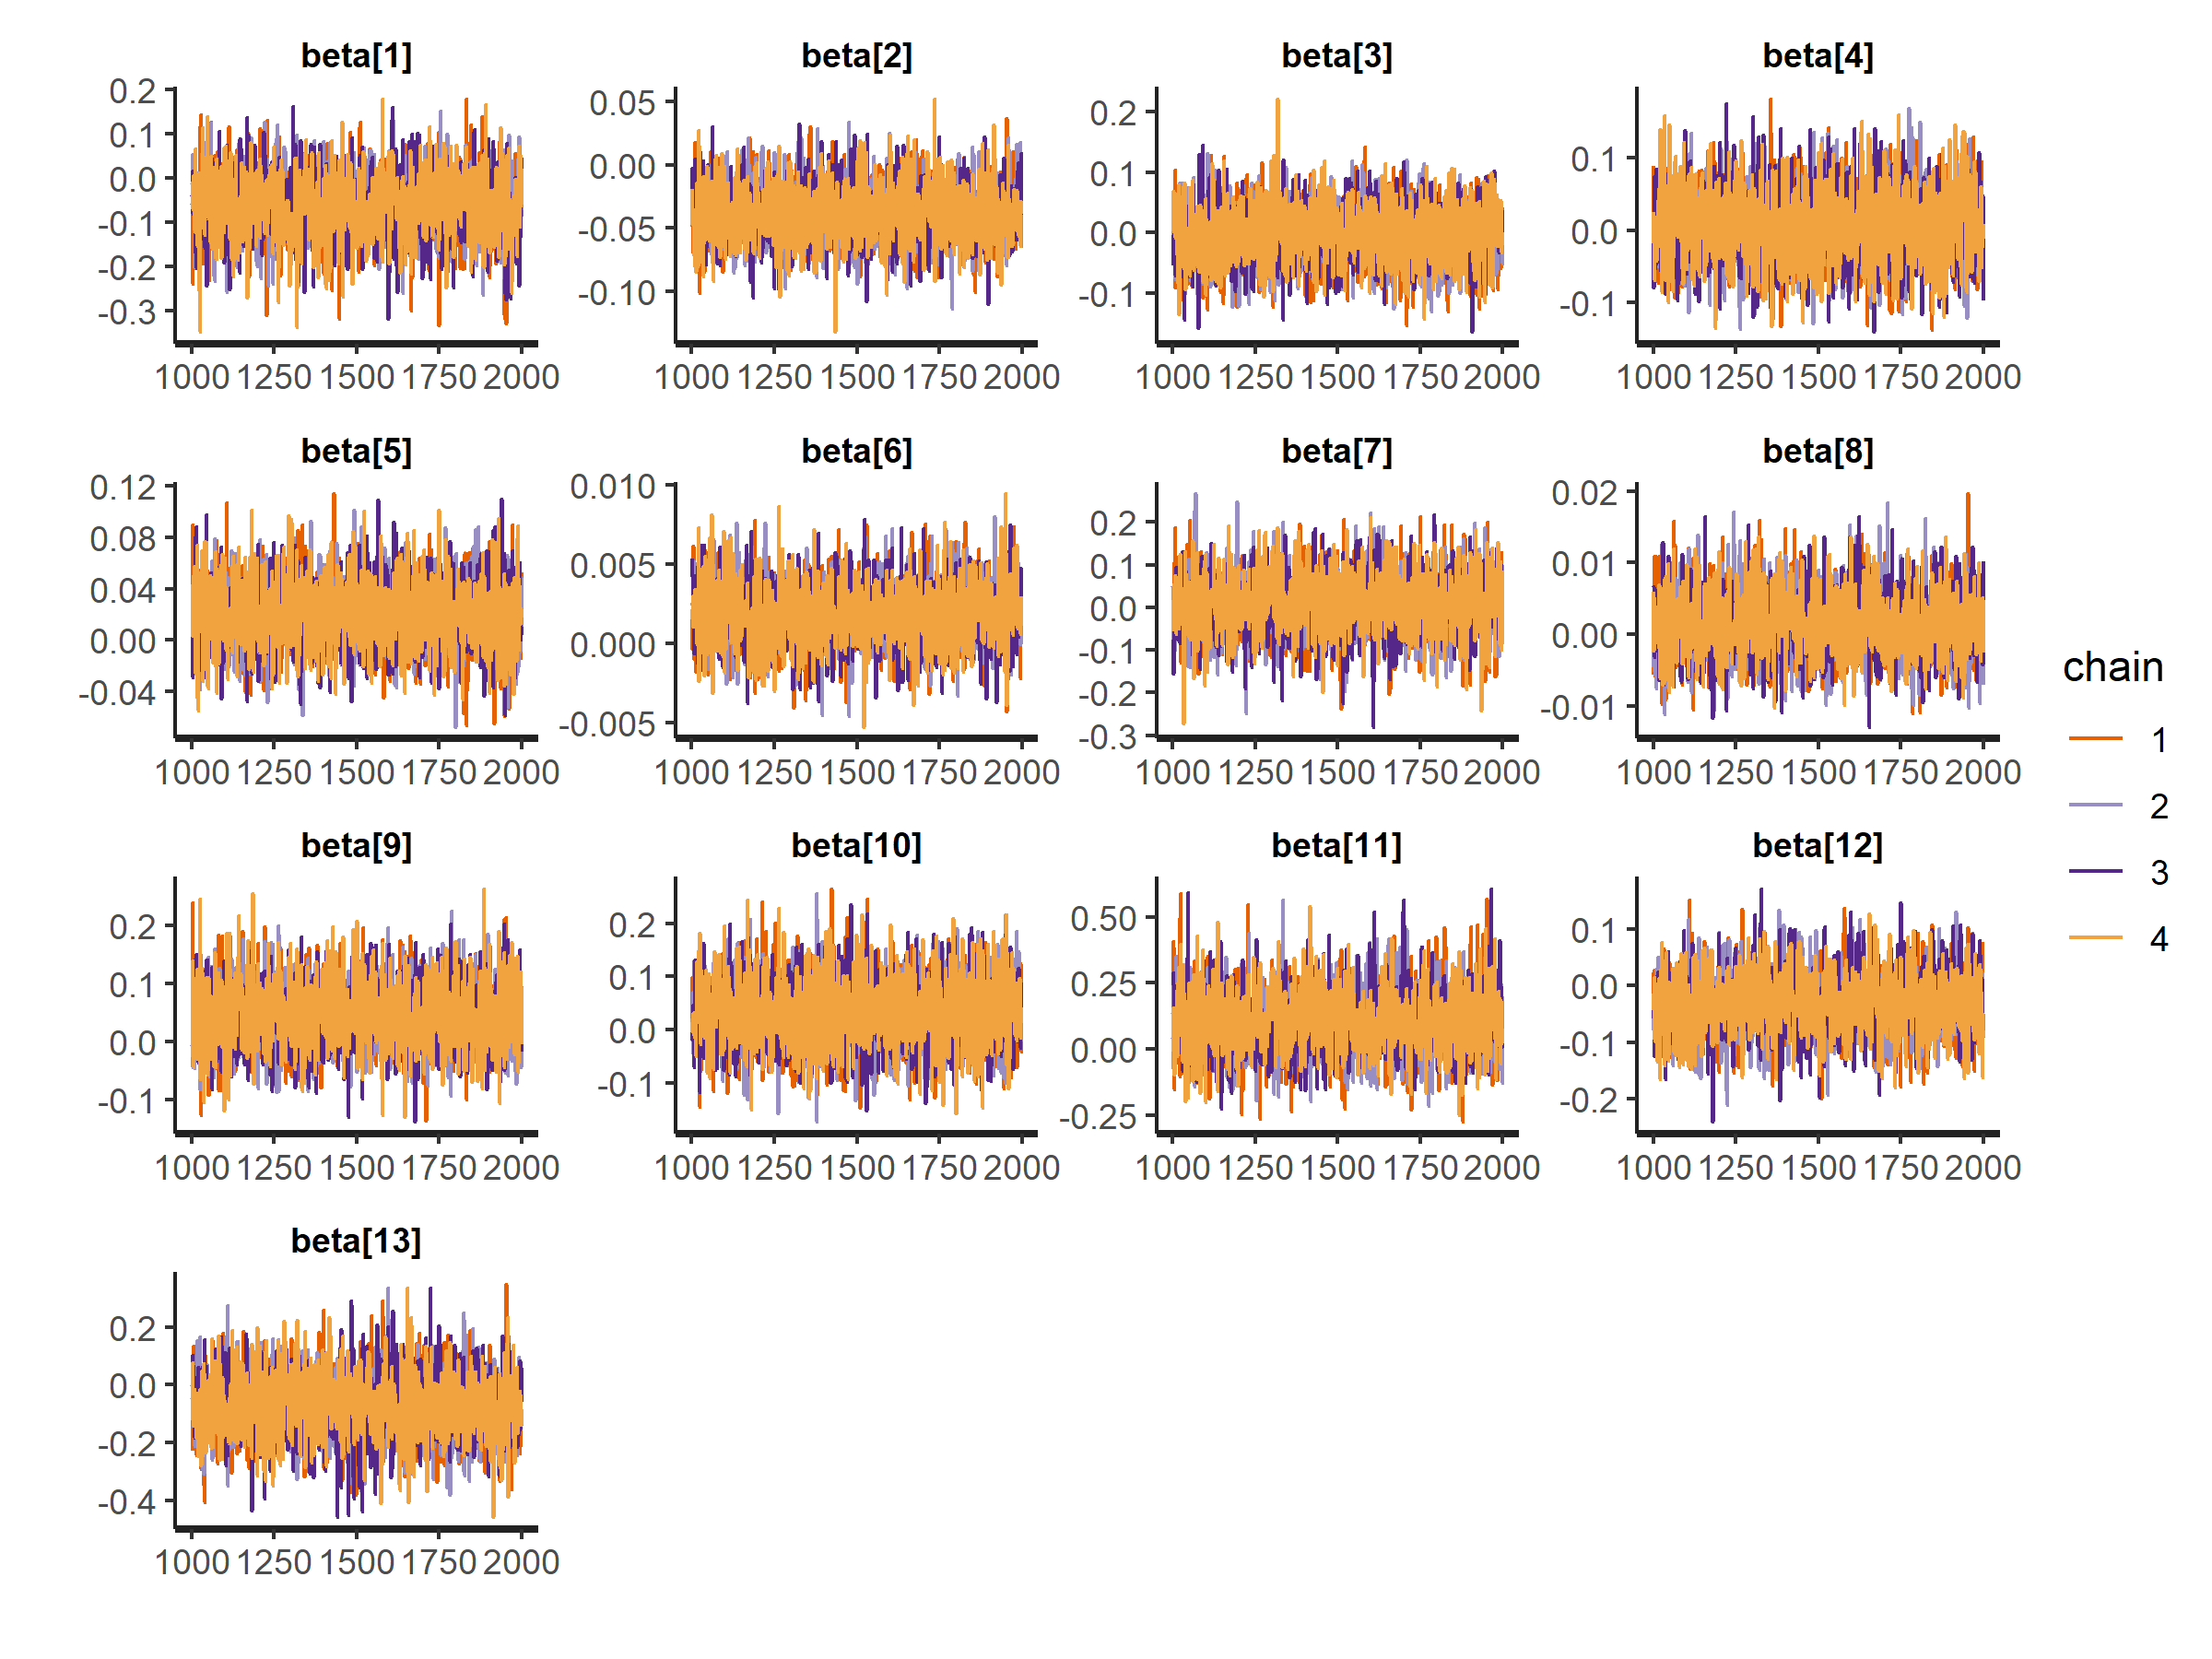
\includegraphics[width=0.95\textwidth]{trace-all-min.png}
	\caption{Traceplot of alliance level parameters in the non-major power sample.}
	\label{fig:trace-all-min}
\end{figure}



\section{Normalizing Allied Capability}

% Justify use of annual normalization
As noted in the paper, I place allied capability in the membership matrix \textbf{Z} on the same scale as the other parameters by normalizing it by year. 
Within each year, I divide the total military spending of allied states by the maximum value, so capability values within each year range from just above zero to one. 
This ensures that allied capability is comparable within years, and that I do not treat more modern alliances as the most capable as raw defense budget sizes increase. 


The choice of this specific normalization is less theoretically informed than using capability itself. 
Therefore, I assessed the use of different normalizations and rescalings for allied capability by comparing model fit. 
I fit three models in addition to the one presented in the paper. 
The first rescaled allied capability by dividing each capability value by the maximum of capability without grouping alliances by year. 
The second rescaled alliance capability by dividing by two standard deviations, which is problematic because it introduces negative capability values. 
The last used total allied CINC scores instead of military spending as an indicator of allied capability, which also facilitates comparisons of allied capability within years. 
CINC scores measure the share of total world military capability each state has in a particular year, so it is useful for comparing allied capability within years \citep{SingerCINC1988}. 


After estimating these three models, I used leave-one-out (LOO) cross validation to assess model fit \citep{Vehtarietal2017}. 
LOO estimates pointwise out-of-sample prediction accuracy using the log-likelihood evaluated at the posterior simulations of the parameter values.\footnote{The widely applicable information criteria (WAIC) produces similar results, but the estimates for the CINC model may be driven by an unusual observation.} 
All diagnostics indicate the LOO results are not driven by unusual observations. 
As with other information criteria, lower values indicate better fit. 

 

\begin{table}[ht]
\centering
\begin{tabular}{rrrrrrrrr}
  \hline
 Allied Capability & elpd\_diff & se\_diff & elpd\_loo & se\_elpd\_loo  \\ 
  \hline
  Normalized by Year & 0.000 & 0.000 & -1159.513 & 184.714 \\ 
  Rescaled by Maximum & -3.165 & 2.643 & -1162.679 & 184.723  \\ 
  Recaled by 2SD & -10.749 & 6.116 & -1170.262 & 184.741  \\ 
  Total Allied CINC & -12.308 & 5.576 & -1171.821 & 184.683  \\ 
   \hline
\end{tabular}
\caption{Leave-one-out cross validation to assess model fit with different rescalings or normalizations of alliance capability. }
\label{tab:loo-zcontents}
\end{table}

\autoref{tab:loo-zcontents} summarizes the assessment of each model using the expected log pointwise predictive density (elpd). 
I use the model from the paper as the comparison model: a negative elpd\_diff implies the normalized model fits the data better. 
The difference also has some uncertainty, which is summarized by the se\_diff column of \autoref{tab:loo-zcontents}. 
The other three models have a negative elpd\_diff compared to the model with normalized capability by year. 
For the models with CINC and rescaling by two standard deviations the difference is large, relative to the se\_diff, so there is a clear preference for the normalized model. 
Normalizing by year provides at best a marginal improvement over a model where capability is rescaled using the maximum. 
Rescaling capability by the maximum produces similar inferences about alliance characteristics, including treaty depth. 



\section{Fake Data Simulation Check}


With any complicated model, simulating fake data and seeing if the model can recover known parameters is essential. 
Fake-data simulation helps validate results from observed data and identify problems. 
This section summarizes results from fitting the multilevel model to fake data.


I simulated a dataset of 2000 t-distributed observations with 50 states observed for 200 years and 100 alliances. 
The outcome has a different scale than the military spending outcome variable, so coefficient values here do not match reported values in the paper.  
I then simulated two state and alliance level variables and a sparse matrix of state membership in alliances. 
Last, I ran the model without evaluating the likelihood, generating a posterior prediction of the outcome based on the fake data.


To check whether the model could recover known parameters, I took the 12th draw of the posterior distribution.
This draw included a simulated outcome for each observation and a set of coefficients. 
I then fit the multilevel model on the simulated outcome values and checked whether the credible intervals contained the corresponding parameter values. 
If a parameter is within the 90\% credible interval, the model captures it. 


The model recovers known parameters with a high degree of accuracy. 
As shown by \autoref{fig:beta-sim-res}, the two credible intervals of the alliance-level regression include the known values.
Credible interval coverage for the variance hyperparameters and $\gamma$ parameters is also acceptable. 


\begin{figure}[htbp]
	\centering
		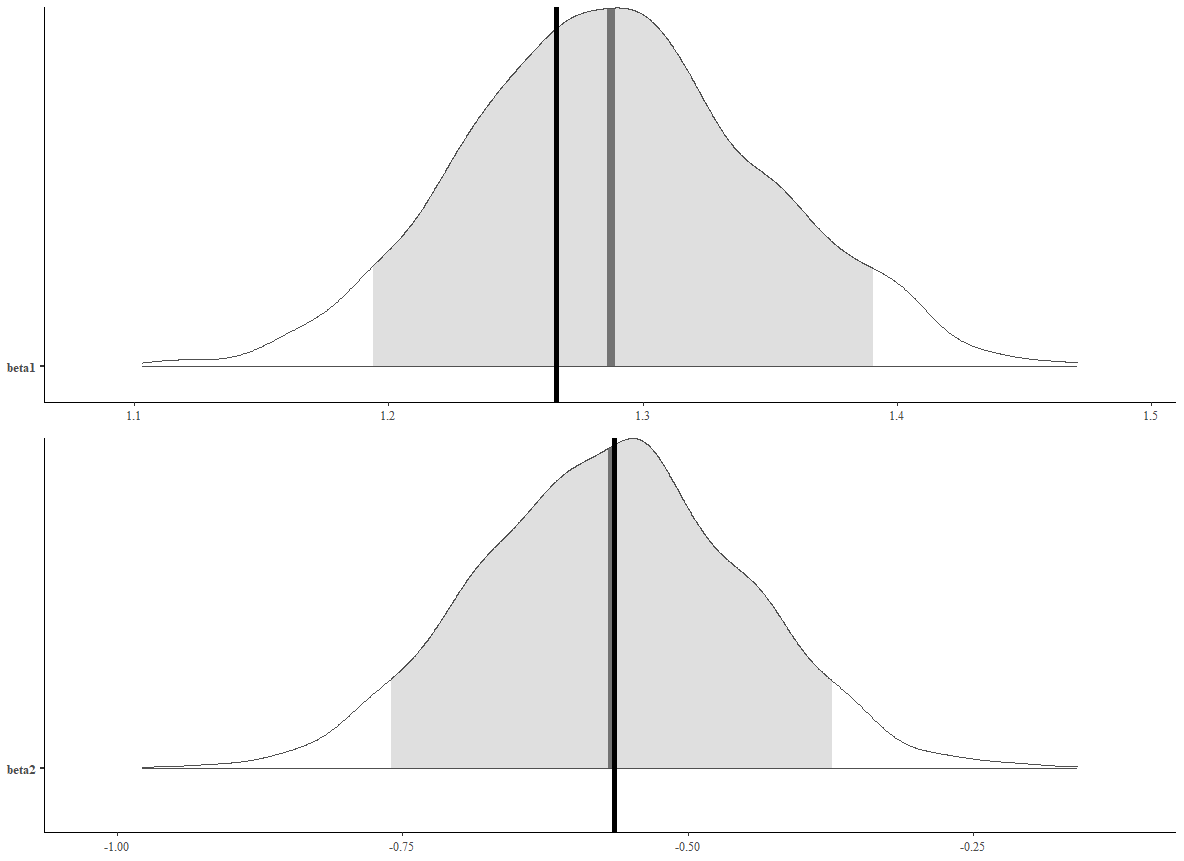
\includegraphics[width=0.95\textwidth]{beta-sim-res.png}
	\caption{Posterior distributions of $\beta$ parameters from fitting multilevel model to fake data. The black vertical line marks the known parameter value, and the grey area is the 90\% credible interval.}
	\label{fig:beta-sim-res}
\end{figure}


 
Even with small multiples, the 100 $\lambda$ parameters are hard to plot, so I offer a descriptive summary here. 
Among the $\lambda$ parameters, 93 of 100 intervals contain the known $\lambda$ value.
Given the large number of parameters and smaller sample, this is acceptable accuracy. 
Even the seven inaccurate confidence intervals were quite close--- all were within .015 of the known parameter.\footnote{Fine margins around these intervals implies that the exact number of accurate $\lambda$ intervals is sensitive to simulation variance.}


In summary, convergence diagnostics and fake data fitting both suggest that the multilevel model works as expected. 
No convergence diagnostics indicate problems exploring the posterior. 
Just as importantly, the model can recover known parameters from fake data. 
The next section provides a check of the results with a different measure of military spending. 




\section{Robustness Check 1: Alternative Measure of Military Spending}

The main findings in the manuscript rely on the Correlates of War military spending. 
Due to reporting issues, definition problems and measurement challenges, other measures of military spending could lead to different results. 
I check the robustness of my results by using \citet{Nordhausetal2012}'s measure of military spending, which combines data from the COW project and the Stockholm International Peace Research Institute (SIPRI). 
\citet{DigiuseppePoast2016} use this measure of military spending in their paper. 


I estimate the same multilevel model on this measure of military spending, which covers from 1949 to 2001. 
This model also checks whether how treaty depth modifies the impact of alliance participation on military spending changes after World War II.
Because the coefficient on a lagged dependent variable in this model is close to one, implying a probable lack of stationarity in levels, I use changes in military spending as the outcome of interest. 


\begin{figure}[htbp]
	\centering
		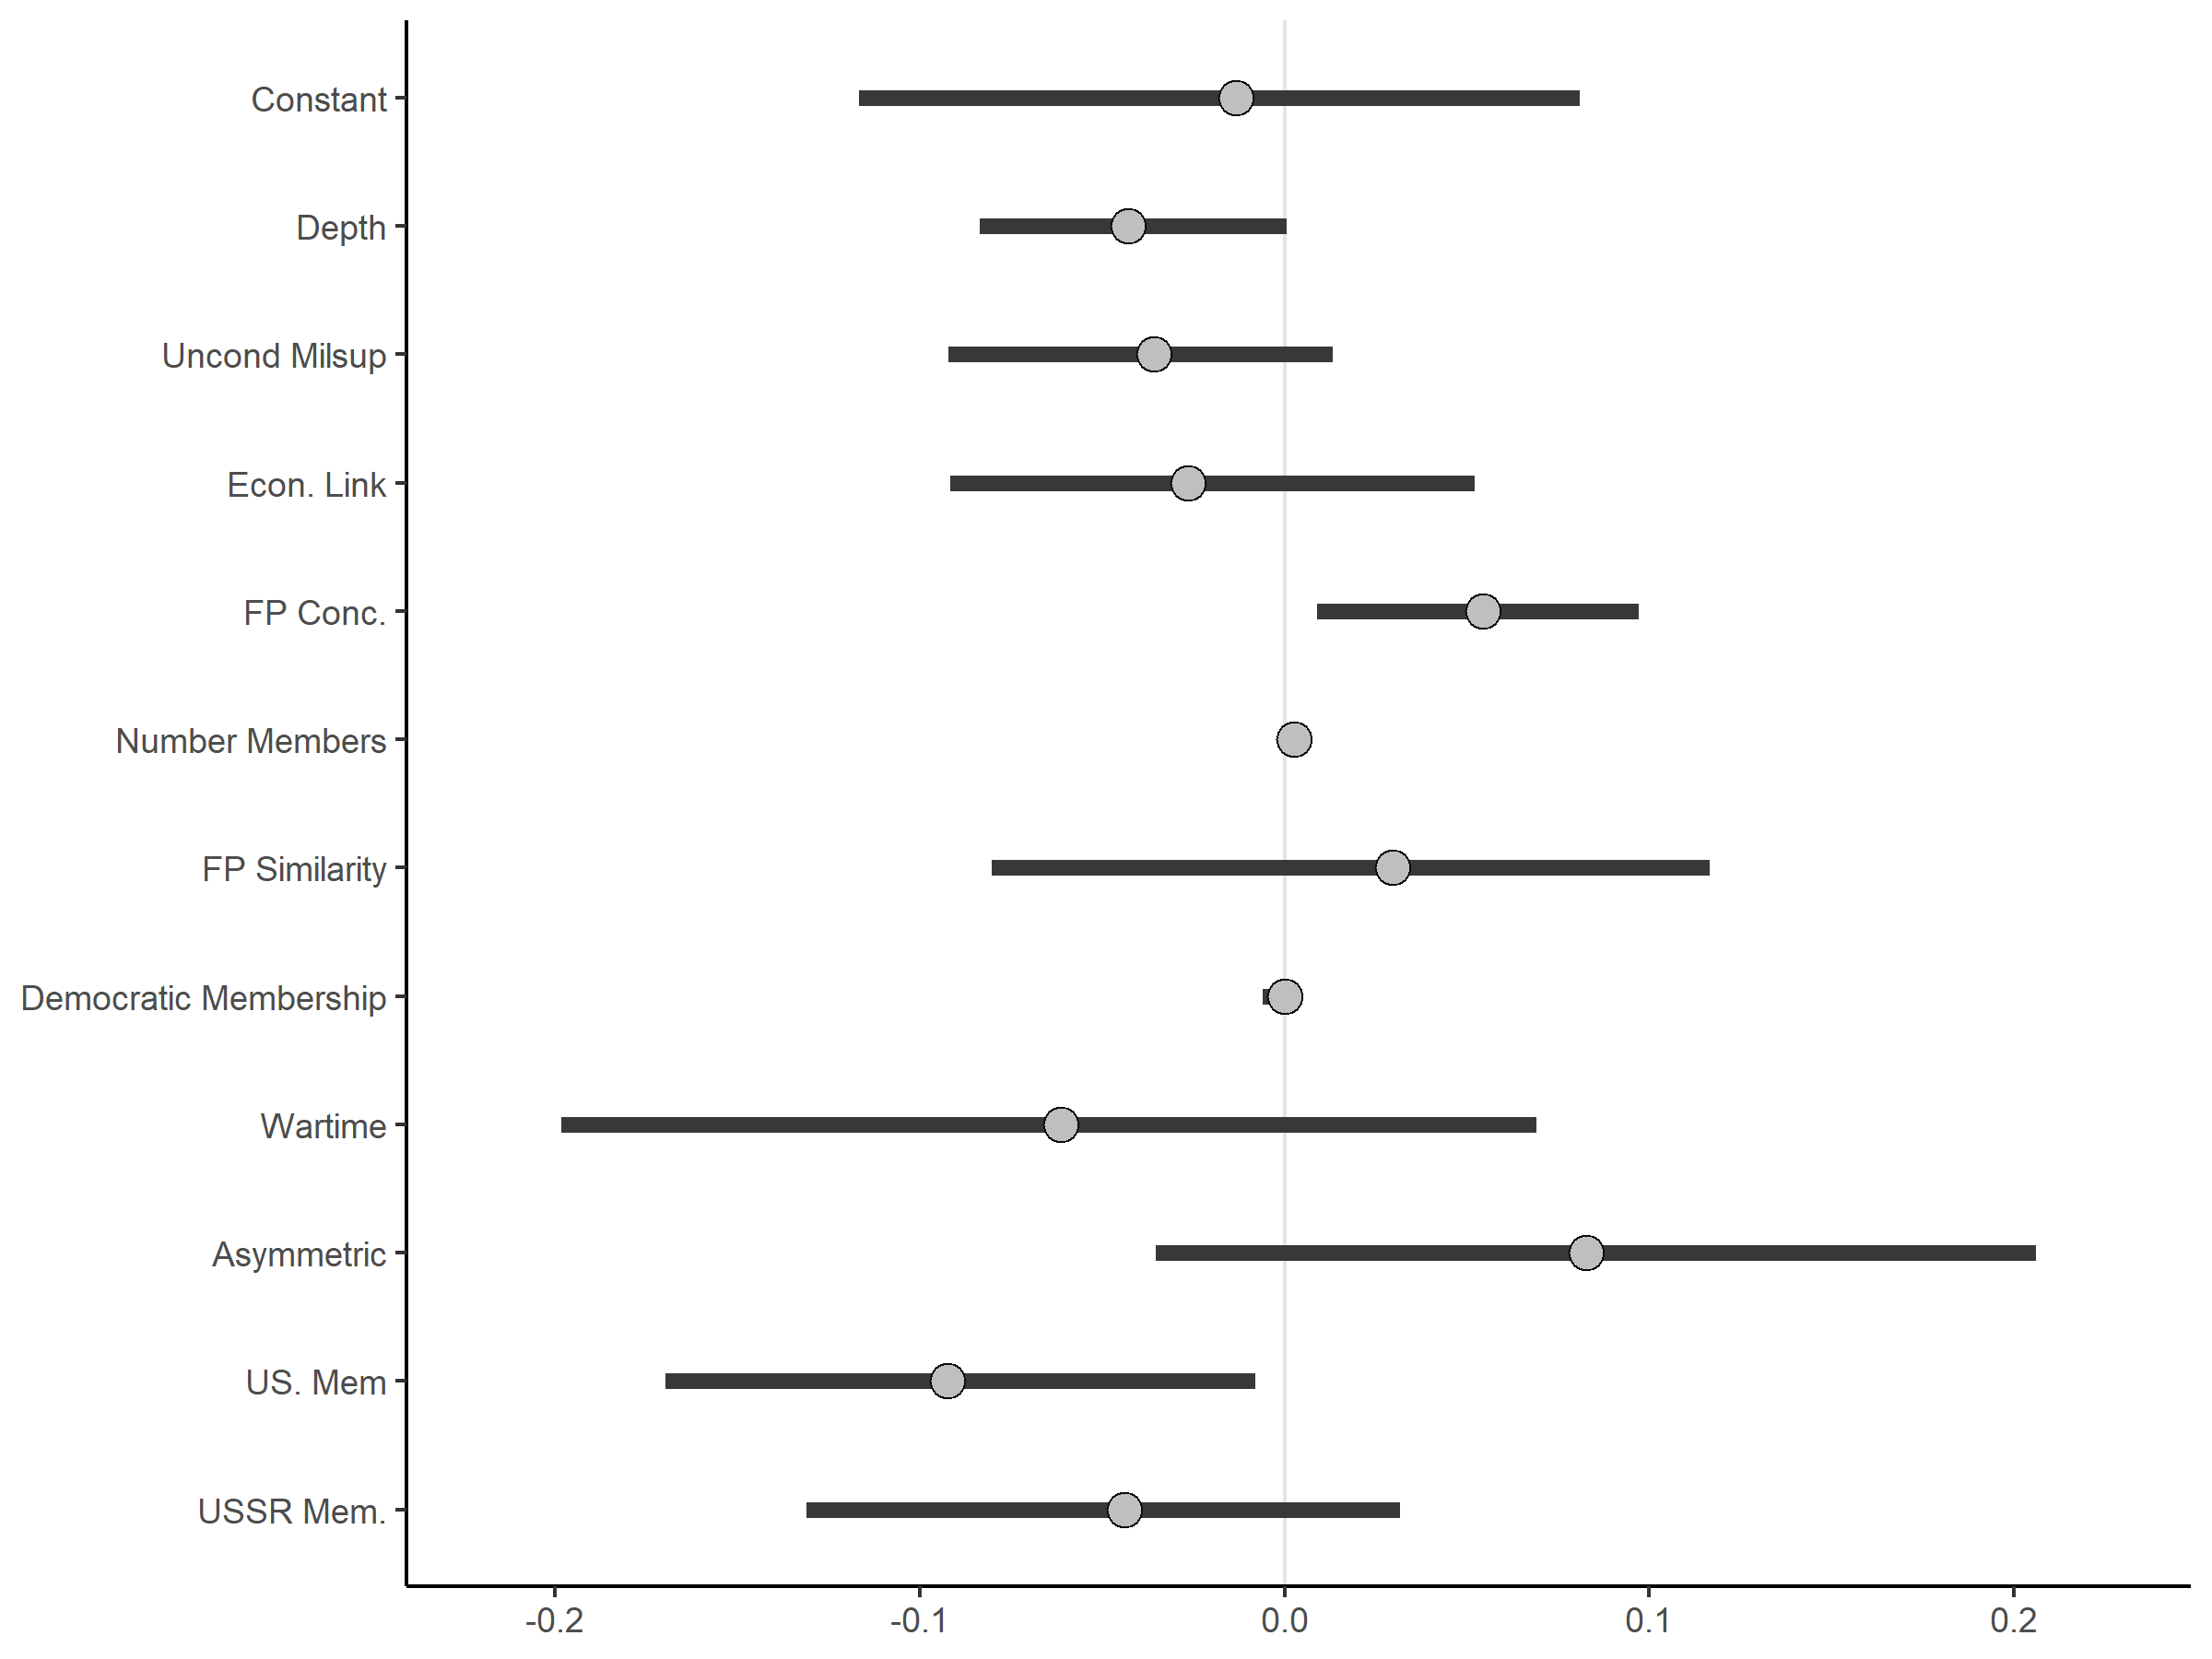
\includegraphics[width=0.95\textwidth]{post45-beta-res.png}
	\caption{90\% credible intervals of the $\beta$ parameters from an analysis of changes in non-major power military spending from 1949 to 2001.}
	\label{fig:post45-beta-res}
\end{figure}


\autoref{fig:post45-beta-res} summarizes the alliance-level regression parameters. 
As with the COW data, the credible interval for treaty depth is negative and does not overlap zero. 
All the parameter estimates are similar in this data, which increases my confidence that the results are not driven by the COW spending data. 

 


\section{Robustness Check 2: Single-Level Regression}

Though the multilevel model best reflects the theory, I also fit some more standard panel data models. 
In what follows, I briefly present results from robust regressions of state-year percentage changes in military spending in the same sample of non-major powers. 
As in the multilevel model, I applied the inverse hyperbolic sine transformation to the outcome. 
In these models, I employ two indicators of alliance depth. 
The first is the average depth of a state's alliances. 
The second is a dummy which equals 1 if a state has at least one alliance with greater than average depth. 
Both variables compare states as the depth of their alliance portfolio shifts. 
In addition to the state-level controls in the multilevel model, I included averages of alliance size and democracy and the log of total allied capability as controls. 


I estimated several models, including robust regressions on all states, non-major powers, and non-major powers in alliances. 
I also applied fixed effects to an OLS model of percentage changes in defense expenditures. 
The estimated association between average treaty depth and military spending changes is summarized in \autoref{fig:single-level-mplot}. 
Results are inconsistent- the average depth measure fails to reject the null without fixed effects. 
The deep alliance dummy coefficient estimate is negative and statistically significant across several samples and model specifications, however. 

\begin{figure}[htbp]
	\centering
		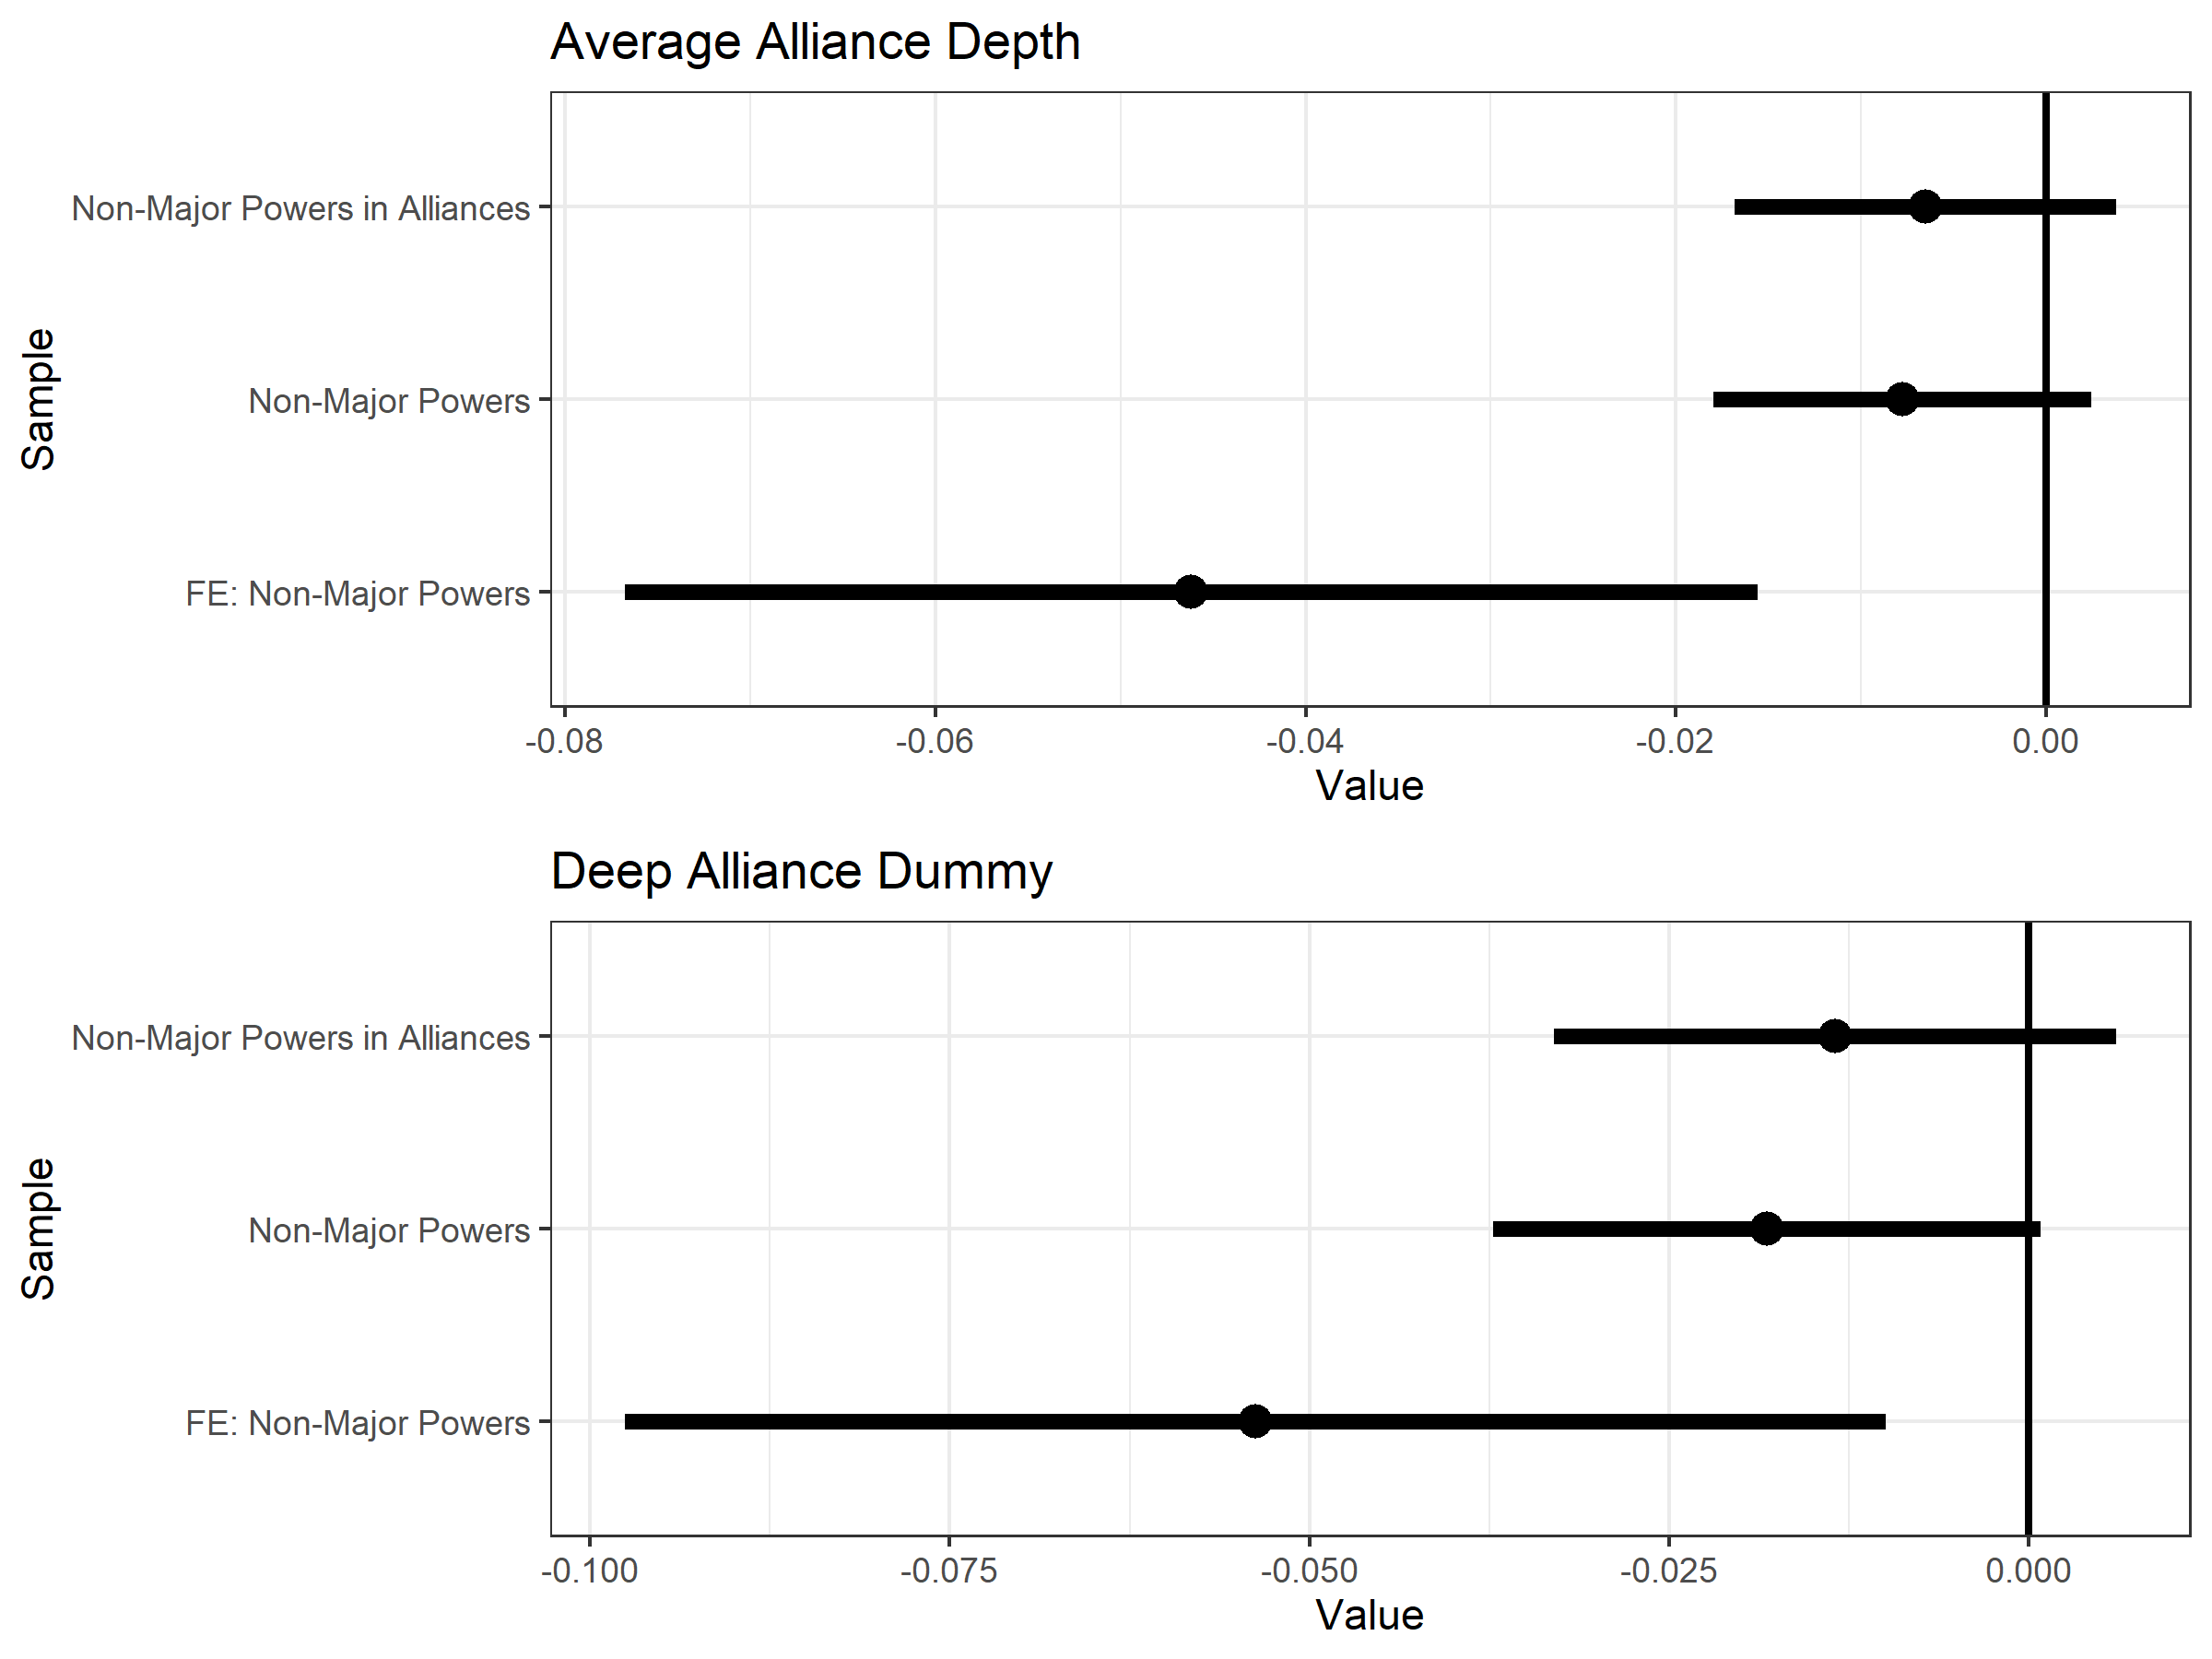
\includegraphics[width=0.95\textwidth]{single-level-mplot.png}
	\caption{Estimated effect of average alliance treaty depth or a dummy indicator of participation in a deep alliance on percentage changes in non-major power military spending.}
	\label{fig:single-level-mplot}
\end{figure}


The analysis of non-major powers in alliances is the best approximation of the multilevel model, as it compares non-major powers with different kinds of alliances. 
Analyzing a sample of all non-major powers includes states with no alliances, with does not match the comparison in the multilevel model. 
To assess the robustness of the coefficient estimate in the sample of non-major powers with alliances, I performed Extreme Bounds analysis. 
Specifically, I present results from \citet{Sala-i-Martin1997}'s method of bounds analysis in \autoref{fig:eba-single-level}. 


\autoref{fig:eba-single-level} shows the distribution of the deep alliance coefficient and an indicator of whether the alliance includes economic agreements. 
Across many specifications, where all regression coefficients are doubtful, the CDF of the deep alliance coefficient has 99\% negative mass. 
Even though the normality assumption is clearly violated, the histogram in \autoref{fig:eba-single-level} shows little evidence having a deep alliance increases percentage changes in military spending. 
The bounds analysis indicates a deep alliance dummy is a robust predictor of percentage changes in military spending across over 1500 single-level model specifications. 


\begin{figure}[htbp]
	\centering
		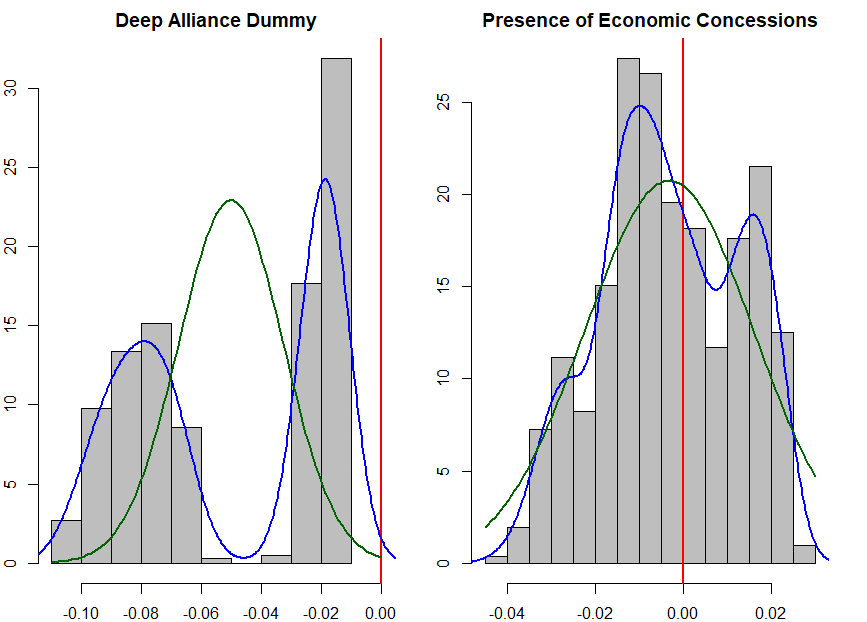
\includegraphics[width=0.95\textwidth]{eba-single-level.png}
	\caption{Histogram of coefficient values for a deep alliance dummy and economic concessions in at least one alliance in a single-level robust regression of non-major powers in alliances.}
	\label{fig:eba-single-level}
\end{figure}




\section{Alternative Measures of Alliance Treaty Depth}

This part of the appendix compares my latent measure of treaty depth with similar measures by \citet{LeedsAnac2005} as well as \citet{BensonClinton2016}. 
I first show that there are important differences between my measure and the military institutionalization measure of \citet{LeedsAnac2005}, but using military institutionalization instead of latent depth generates similar inferences. 
Then I move to the conceptual differences between my latent measure and that of \citet{BensonClinton2016}.


\subsection{Leeds and Anac 2005}


\citet{LeedsAnac2005} create an ordinal measure of alliance treaty depth to study whether alliance institutionalization improves treaty reliability and performance. 
They argue that commitments of an integrated military command, common defense policy, or any sort of basing rights generate high military institutionalization. 
Official contact between military officials, formal organizations, training or technology, subordination of forces, or specific contributions reflect moderate institutionalization. 
If at least one factors is present, the offensive or defensive alliance is coded as the corresponding level of institutionalization. 
This assumes that alliances with multiple sources of depth as just as deep/institutionalized as alliances with one factor and understates the amount of variation in alliance treaty depth. 


\begin{figure}[htbp]
	\centering
		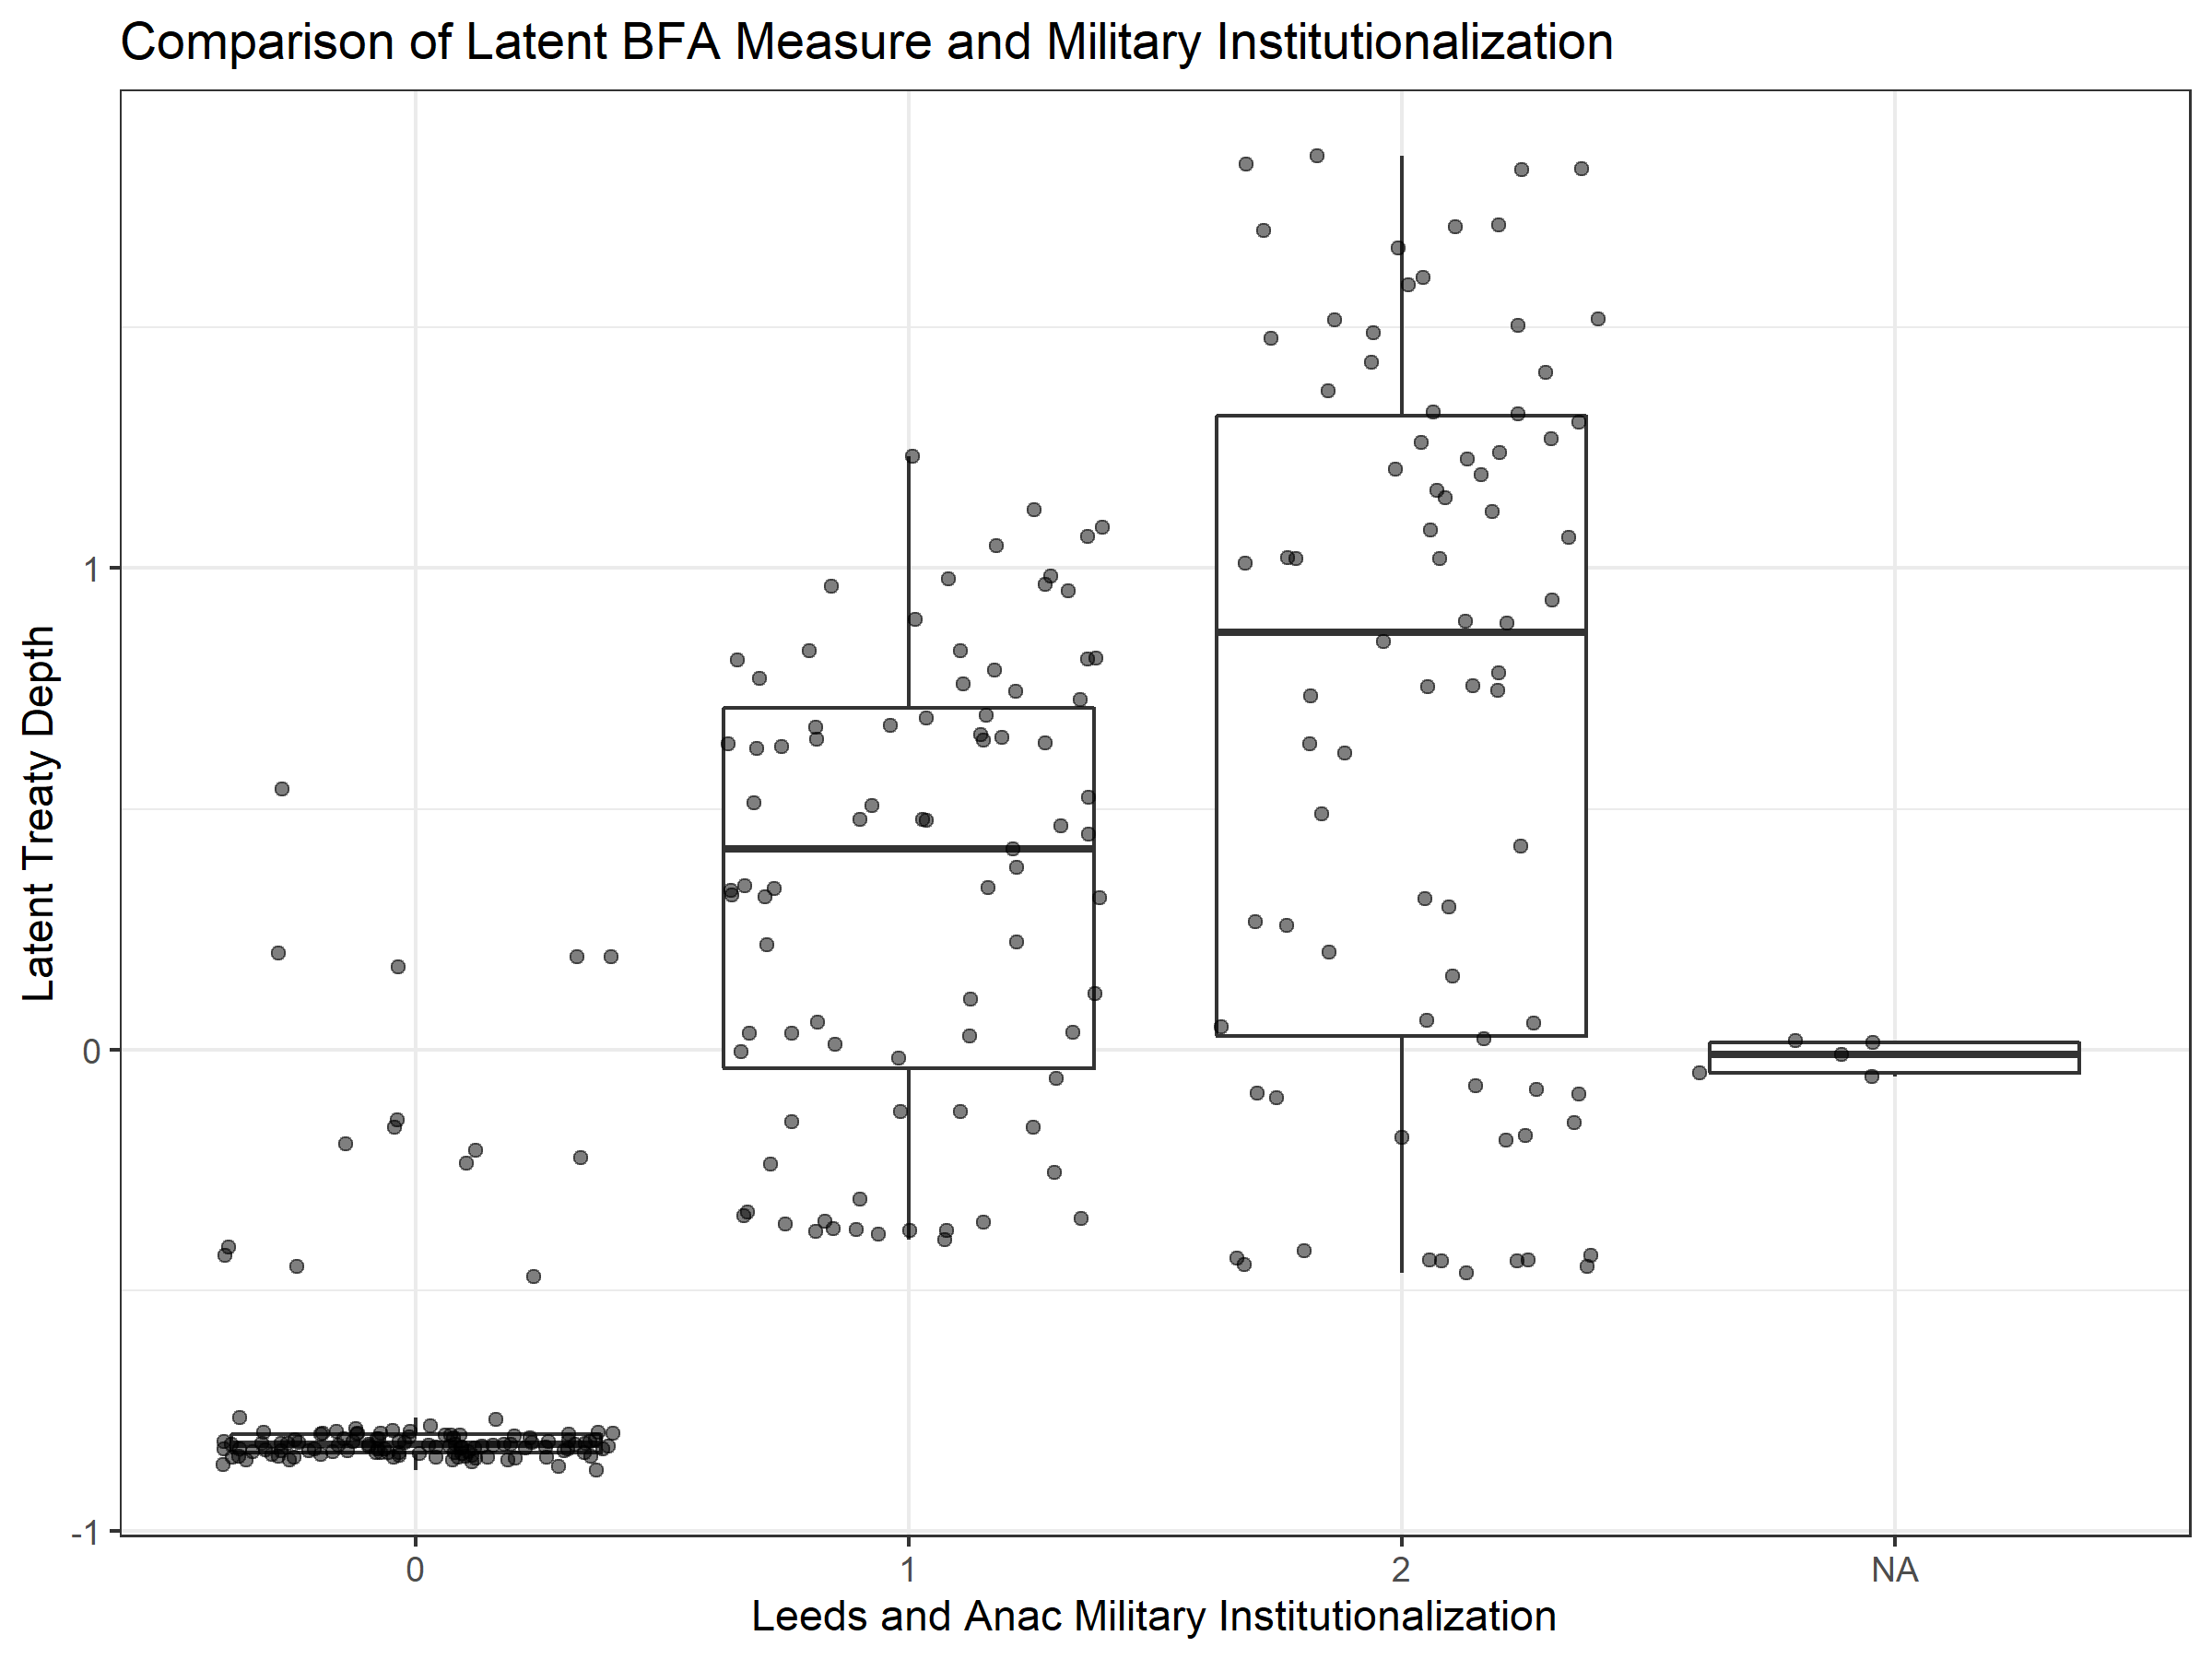
\includegraphics[width=0.95\textwidth]{leeds-anac-comp.png}
	\caption{Scatter plot of latent treaty depth across the values of military institutionalization from \citet{LeedsAnac2005}. The box plots summarize the distribution of latent treaty depth within each category of military institutionalization.}
	\label{fig:leeds-anac-comp}
\end{figure}


As \autoref{fig:leeds-anac-comp} shows, this ordinal measure and my latent measure make fairly similar conclusions and are positively correlated. 
The deepest alliances on the latent measure also have the highest military institutionalization score. 
There are substantial differences within each category and overlap in the latent measure across the categories, however. 
For example, some alliances that \citet{LeedsAnac2005} assign a moderate institutionalization score have far more depth than alliances with high institutionalization scores because these alliance treaties include multiple sources of depth. 


There are a few alliances where my measure makes a marked departure from Leeds and Anac. 
Frist, there are some alliances with no institutionalization that my measure assigns some depth to. 
These alliances are primarily the result of companion military agreements, which I include as a source of depth in addition to Leeds and Anac's variables. 
Second, Leeds and Anac assign missing values to some institutionalization scores if all sources of high or moderate depth are missing, which is a reasonable choice with their measurement strategy.
My latent measure assigns some depth to these treaties, because it ignores missing data on a subset of variables. 
Missing values have no effect on the depth score, but observed values contribute. 


Because the military institutionalization measure captures a similar concept, but has some differences, a robustness check is necessary. 
To check the robustness of my results, I implemented the same multilevel model of non-major power military spending, but replaced the mean latent treaty depth variable with the institutionalization measure. 
\autoref{tab:milinst-res} summarizes the results. 


\begin{table}[ht]
\centering
\begin{tabular}{rrrrrrr}
  \hline
 & mean & sd & 5\% & 95\% & n\_eff & Rhat \\ 
  \hline
Constant & 0.003 & 0.058 & -0.094 & 0.096 & 2688.743 & 1.001 \\ 
  Military Inst. & -0.035 & 0.024 & -0.075 & 0.004 & 3960.366 & 1.000 \\ 
  Uncond. Milsup. & -0.018 & 0.042 & -0.087 & 0.051 & 3450.201 & 1.000 \\ 
  Econ. Link & 0.015 & 0.049 & -0.066 & 0.096 & 3056.525 & 1.000 \\ 
  FP Conc. & 0.025 & 0.025 & -0.017 & 0.066 & 4115.104 & 1.000 \\ 
  Number Members & 0.002 & 0.002 & -0.001 & 0.004 & 3696.671 & 1.000 \\ 
  FP Similarity & -0.005 & 0.065 & -0.110 & 0.105 & 2697.860 & 1.001 \\ 
  Democratic Membership & 0.001 & 0.004 & -0.006 & 0.008 & 3134.146 & 1.000 \\ 
  Wartime & 0.047 & 0.051 & -0.037 & 0.132 & 3879.252 & 1.000 \\ 
  Asymmetric & 0.056 & 0.059 & -0.037 & 0.155 & 2909.115 & 0.999 \\ 
  US. Mem & -0.033 & 0.049 & -0.112 & 0.049 & 2617.047 & 1.000 \\ 
  USSR Mem. & -0.079 & 0.098 & -0.237 & 0.083 & 3185.998 & 1.000 \\ 
  sigma Alliances & 0.143 & 0.054 & 0.060 & 0.234 & 914.843 & 1.003 \\ 
   \hline
\end{tabular}
\caption{Results from an analysis that replaces the latent measure of treaty depth with an ordinal measure of military institutionalization from \citet{LeedsAnac2005}. The negative correlation between treaty depth and the impact of alliance participation on military spending remains.}
\label{tab:milinst-res}
\end{table}


The same finding about treaty depth holds when the analysis uses military institutionalization in place of mean latent treaty depth. 
Military institutionalization and the impact of alliance participation on military spending are negatively correlated. 
93\% of the posterior probability in the depth coefficient is negative, which matches Hypothesis 3. 


\autoref{fig:milinst-lambda} helps assess Hypotheses 1 and 2. 
Among alliances with no institutionalization, most treaties have a positive effect. 
Alliances with moderate institutionalization have mixed effects. 
Last, participation in alliances with high institutionalization tends to reduce military spending. 
This corresponds to the predictions of Hypotheses 1 and 2. 
The trend across military institutionalization is less clear than with the latent measure of treaty depth, however.
This is probably because the military institutionalization measure lumps diverse alliances into coarse bins. 


\begin{figure}[htbp]
	\centering
		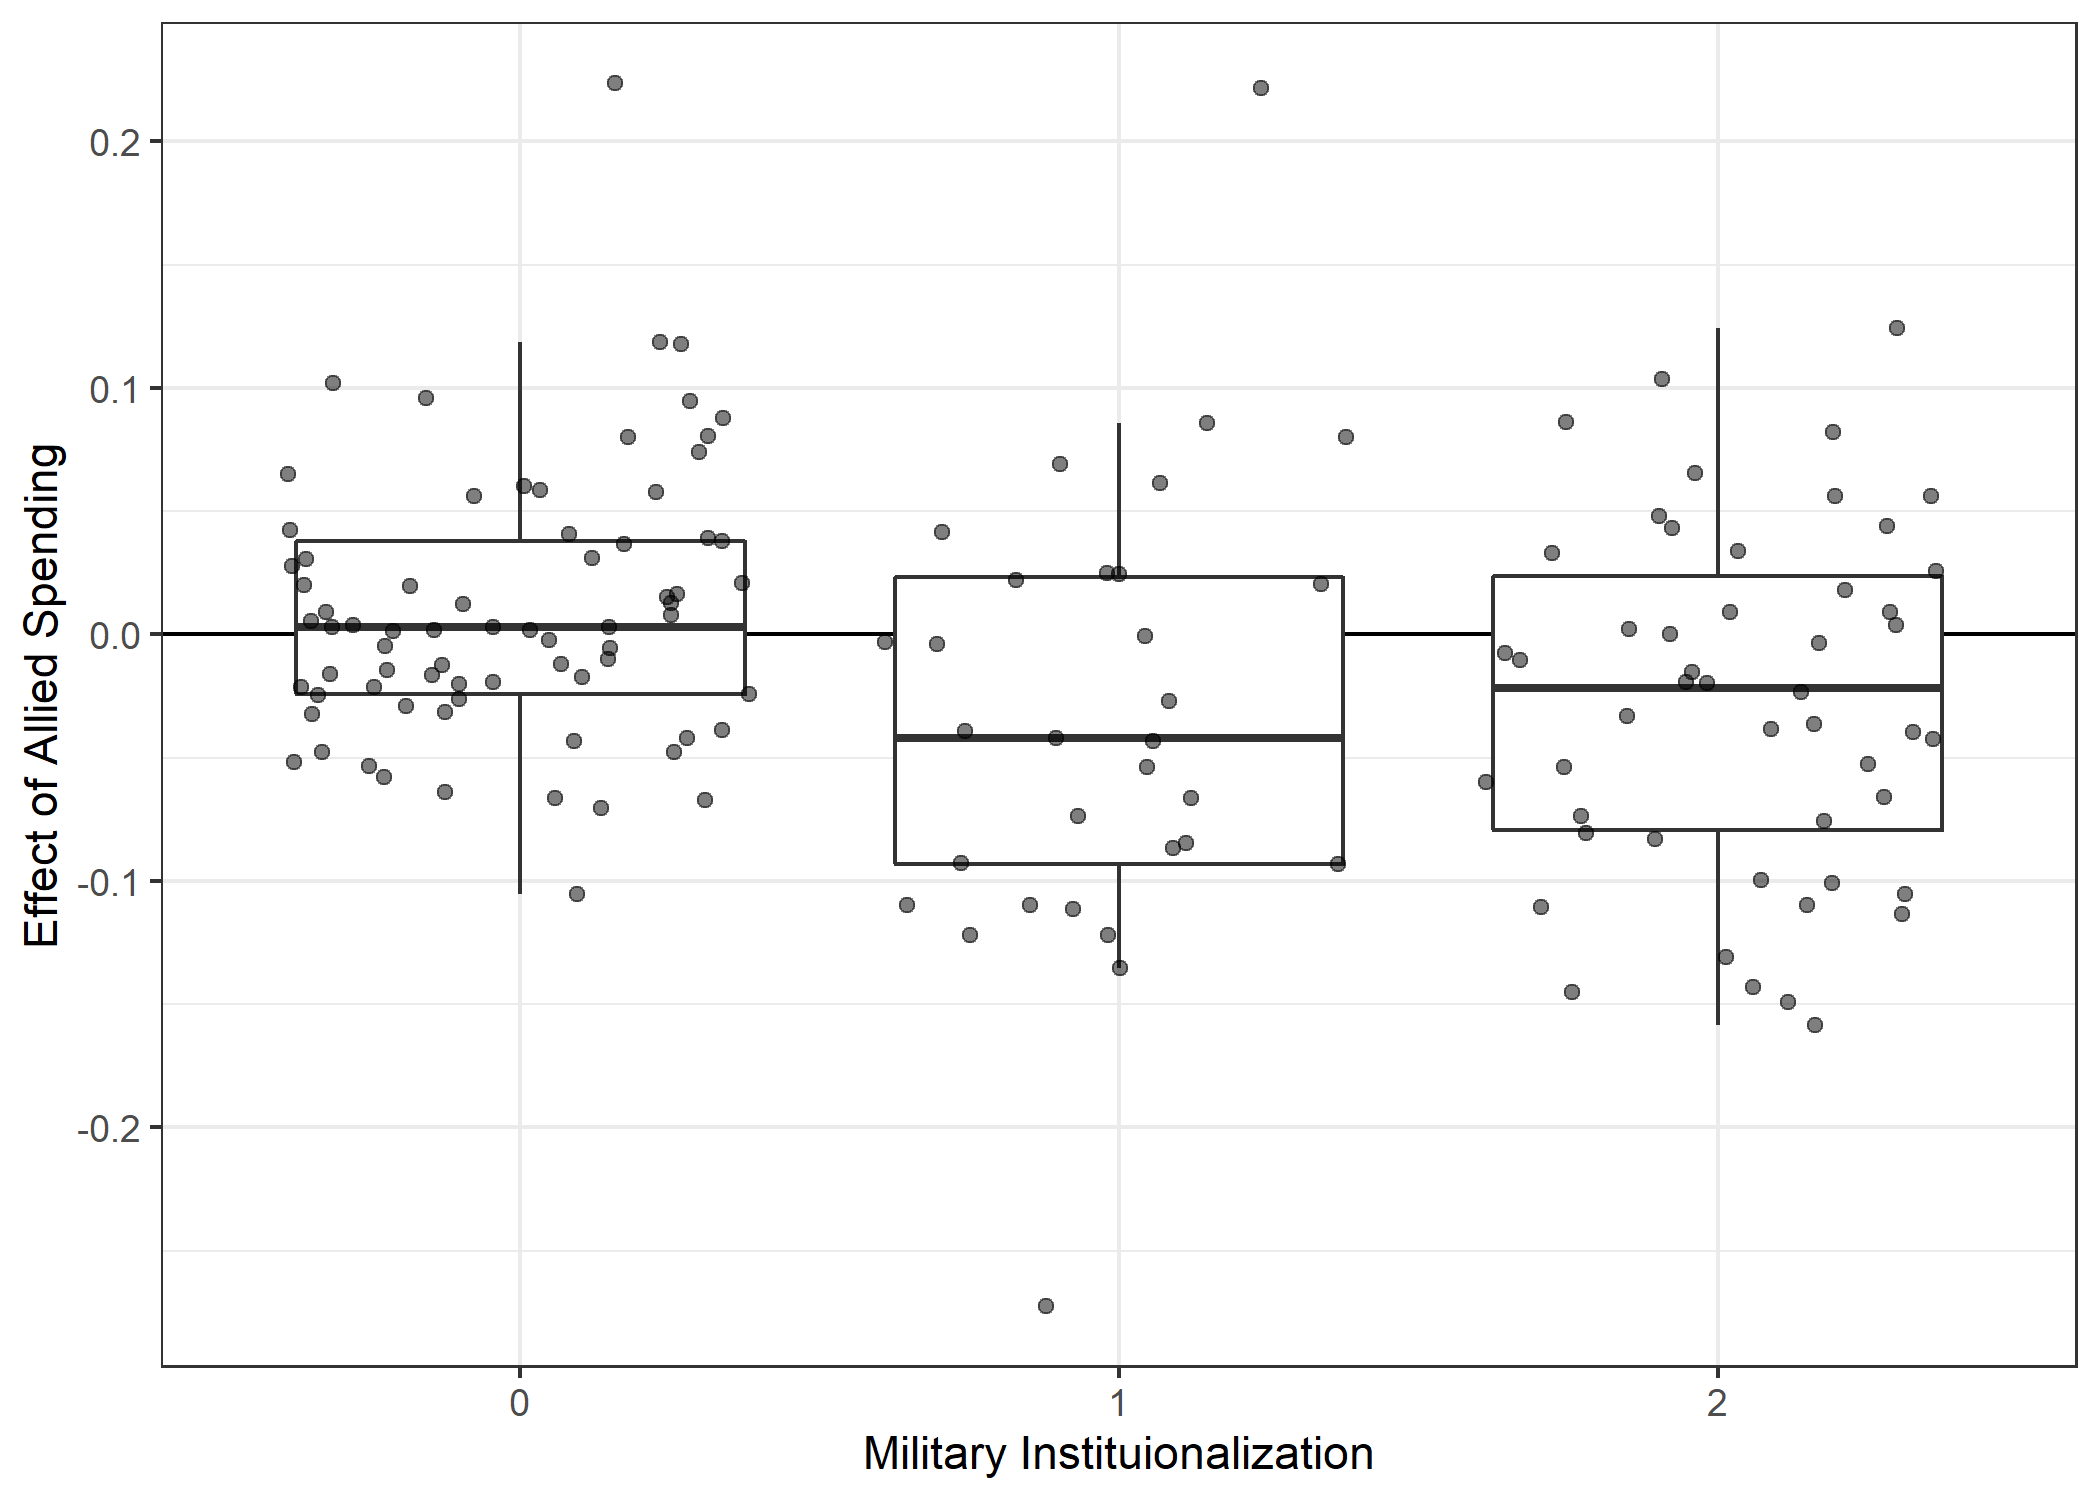
\includegraphics[width=0.95\textwidth]{milinst-lambda.png}
	\caption{Scatter plot of $\lambda$ parameters against the values of military institutionalization. The box plots summarize the distribution of points within in each military institutionalization value. All points are jittered to make the plot more legible.}
	\label{fig:milinst-lambda}
\end{figure}



\subsection{Benson and Clinton 2016}


\citet{BensonClinton2016} use a latent variable model to estimate alliance scope, depth and capability. 
I do not use their measure of depth because it captures a different concept, and thus diverges from my aims in this project. 
Benson and Clinton define depth as the general costliness of alliance obligations, which leads them to include neutrality pacts. 
I define depth as military coordination and cooperation and am only interested in alliances with active military support. 
My focus on defensive and offensive alliances follows existing scholarship on alliance participation and military spending.
These differences, coupled with my use of a different estimator, mean that we draw different conclusions about the factor loadings and the latent depth scores.


% including neutrality pacts changes the comparison category in the measurement model, essentially
Benson and Clinton seek to measure alliance treaty characteristics broadly, so they include neutrality pacts in their data. 
There is an understandable choice, but it means their measure diverges from the my argument, which focuses on alliances with military support. 
Including neutrality pacts in the measurement model alters inferences about the factor loadings. 
Neutrality pacts are qualitatively different, because peacetime coordination is not focused on ensuring the delivery of military support. 


In Benson and Clinton's measure, neutrality pacts have very little depth, which is unsurprising.
Neutrality is less costly in general.  
Only a few alliances with only neutrality obligations have any depth, as \autoref{fig:bc2016-neutral} shows.  

\begin{figure}[htbp]
	\centering
		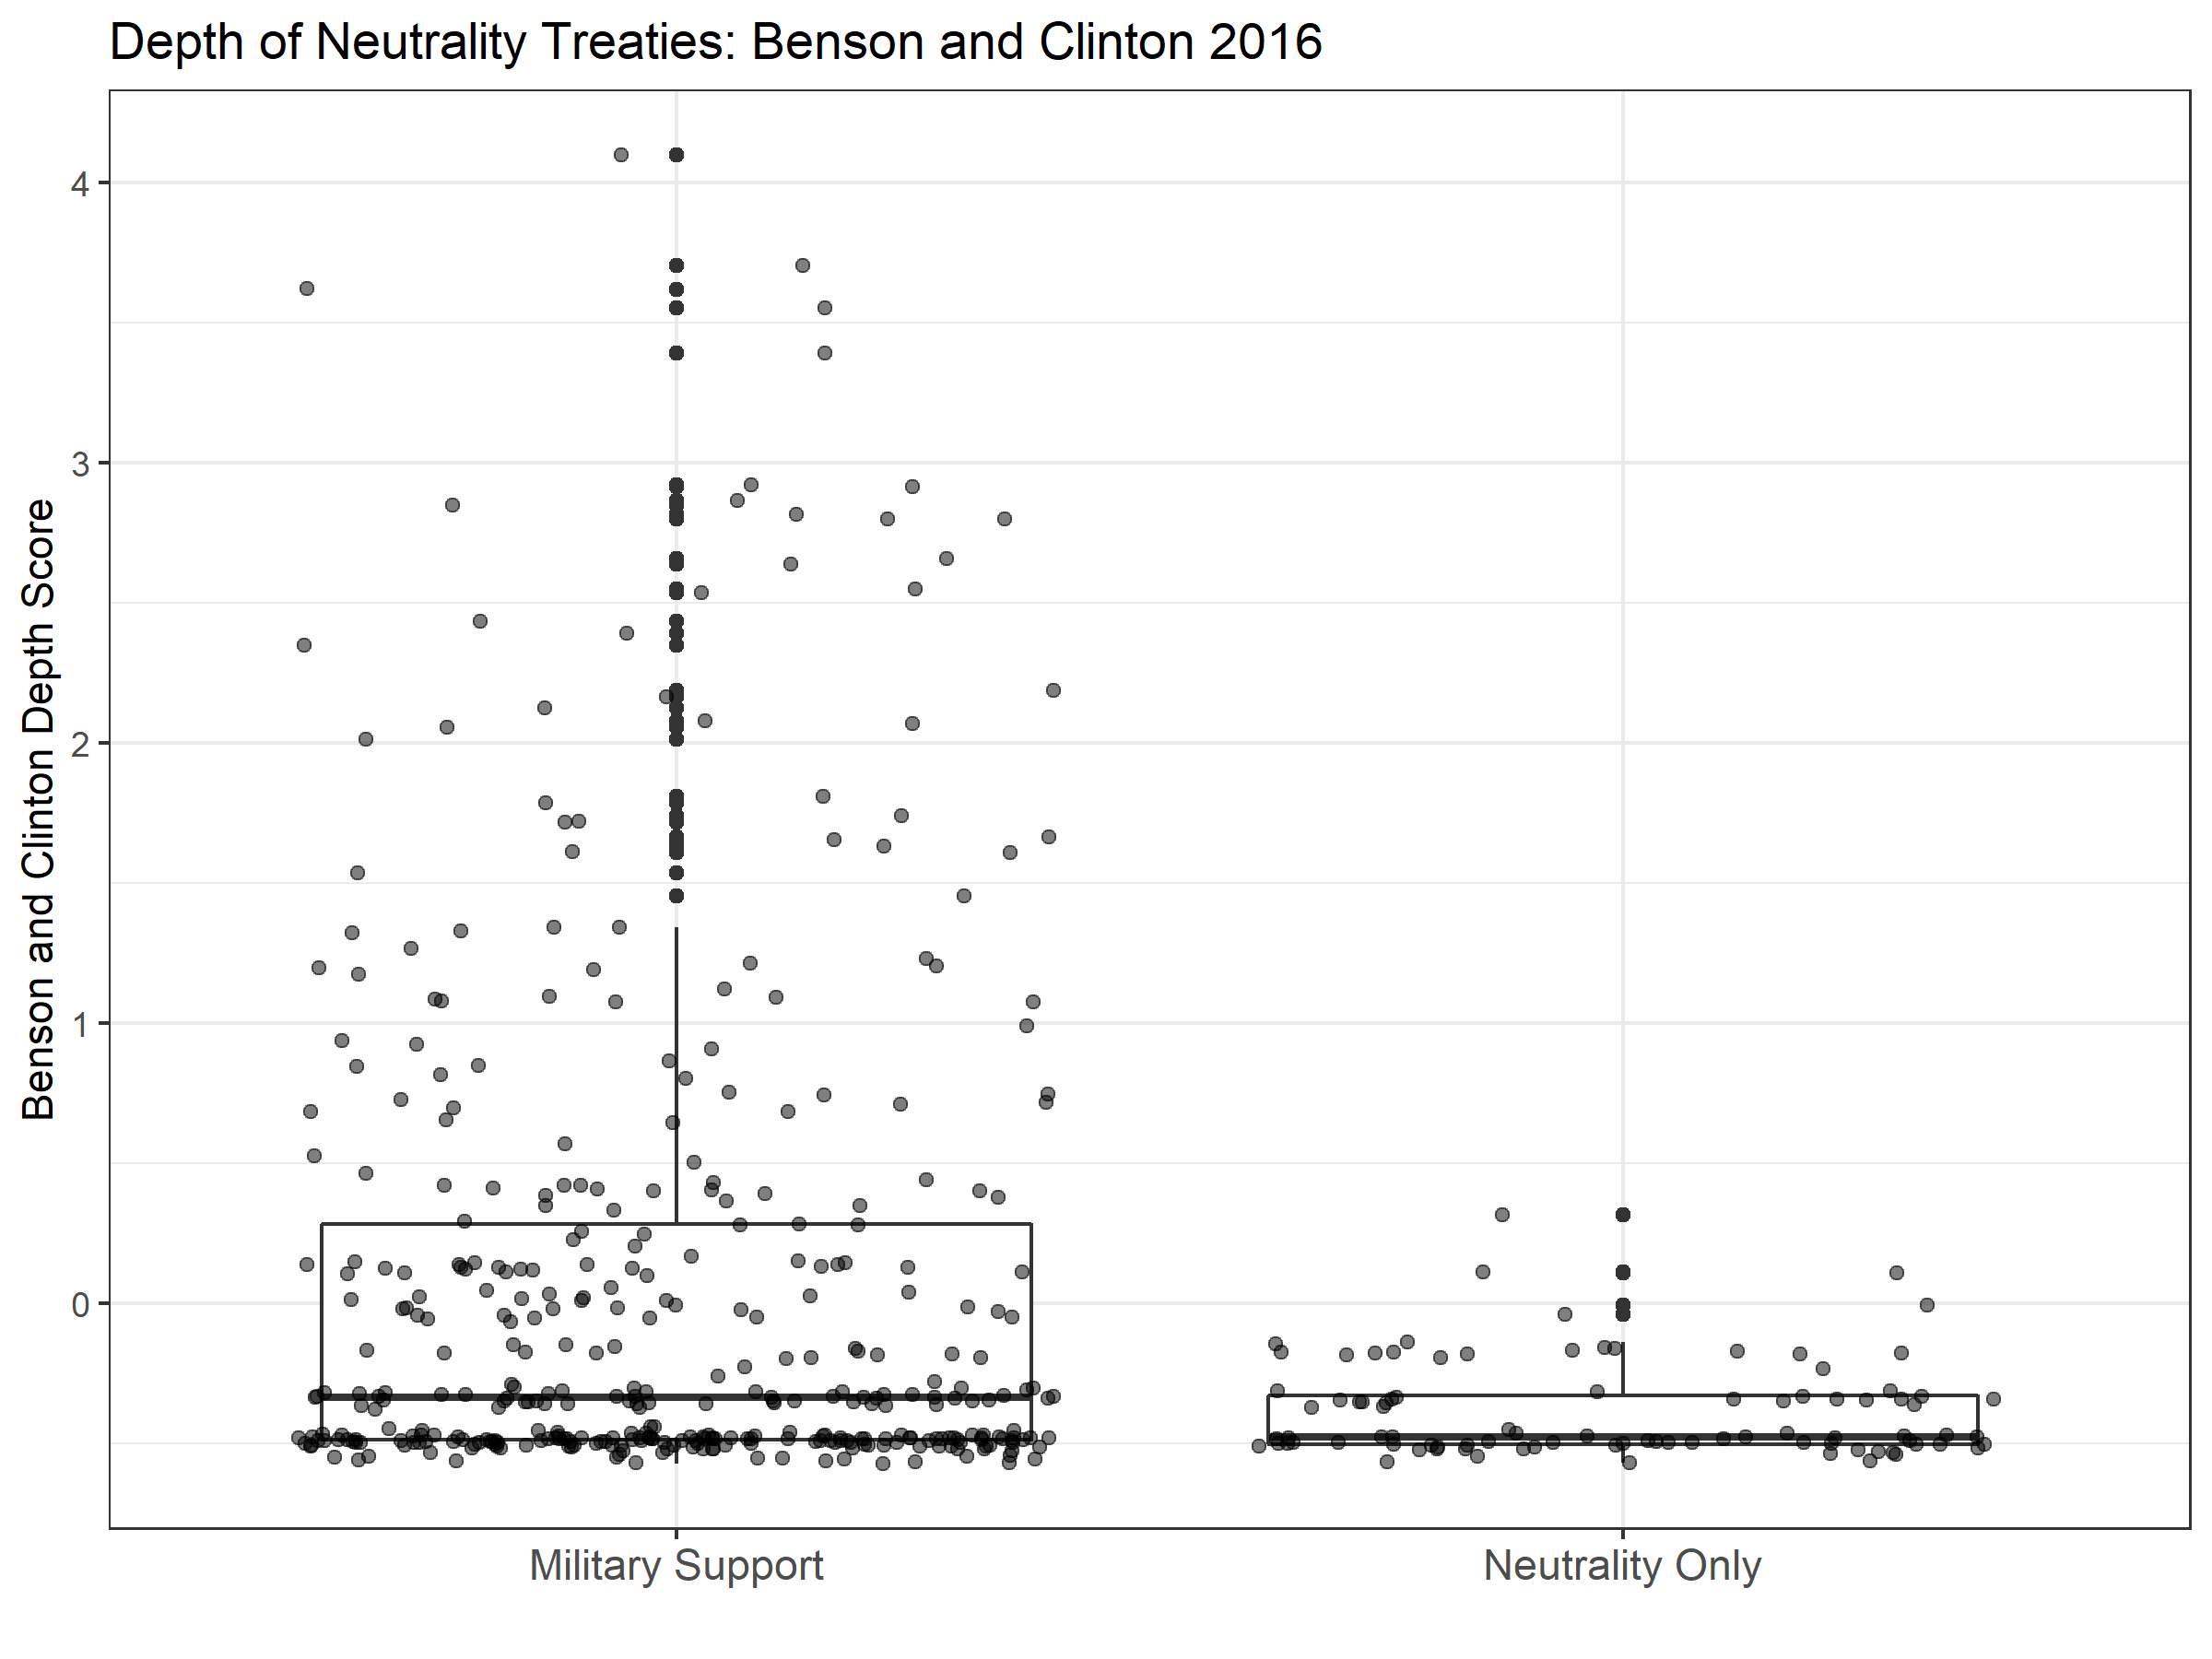
\includegraphics[width=0.95\textwidth]{bc2016-neutral.png}
	\caption{Comparison of Benson and Clinton's depth measure among alliances with only neutrality obligations and alliances with active offensive or defensive support. The box plots summarize the distribution of alliance depth within each group of alliances. All points are jittered to make the plot more legible.}
	\label{fig:bc2016-neutral}
\end{figure}


In Benson and Clinton's model, limited alliances with neutrality promises are a sort of reference category for military alliances. 
Neutrality pacts have limited depth, but they will inform inferences about the depth of alliances with offensive or defensive promises. 
As with other statistical models, inferences from measurement models can be sensitive to different reference categories. 
By including neutrality pacts, Benson and Clinton's model compares alliances with generally limited obligations to more costly military support pacts.


Again, Benson and Clinton's decision to measure the depth of neutrality pacts is not a problem for their paper. 
It limits my ability to apply their measure to this project, however. 
I do not address neutrality pacts in my argument, so my measure of depth must focus on offensive and defensive alliances. 
My emphasis on defense pacts leads to a more narrow focus on military cooperation.
Coupled with my use of an estimator that breaks problematic correlations between the latent variables and dependence structure \citep{Murrayetal2013}, I draw different conclusions about the factor loadings and depth of different alliance treaties. 


% differences in loadings and estimator have important consequences for depth scores
\autoref{fig:bc-2016-comp} describes the key differences between my latent measure of depth and Benson and Clinton's measure.
On the top panel, I look at differences in the factor loadings across the two models.\footnote{Recall that I removed economic aid and secrecy from the observed data in my measure, because they are distinct from military cooperation.} 
Benson and Clinton break the policy coordination variable into military contact and common defense policy, but I treat this as an ordinal variable, which is the largest source of depth.\footnote{The military contact variable on which the policy coordination score is based gives alliances that require wartime military contact a score of one, scores treaties with peacetime military contact as a two, and assigns alliances with defense cooperation a score of three. There is a clear progression in the extent of policy coordination required as this variable increases.}
I also find larger correlations between formal organization and integrated military command and latent depth than Benson and Clinton.
It is harder to distinguish between other loadings, but Benson and Clinton's measure assigns marginally more weight to military aid and basing rights.  


\begin{figure}[htbp]
	\centering
		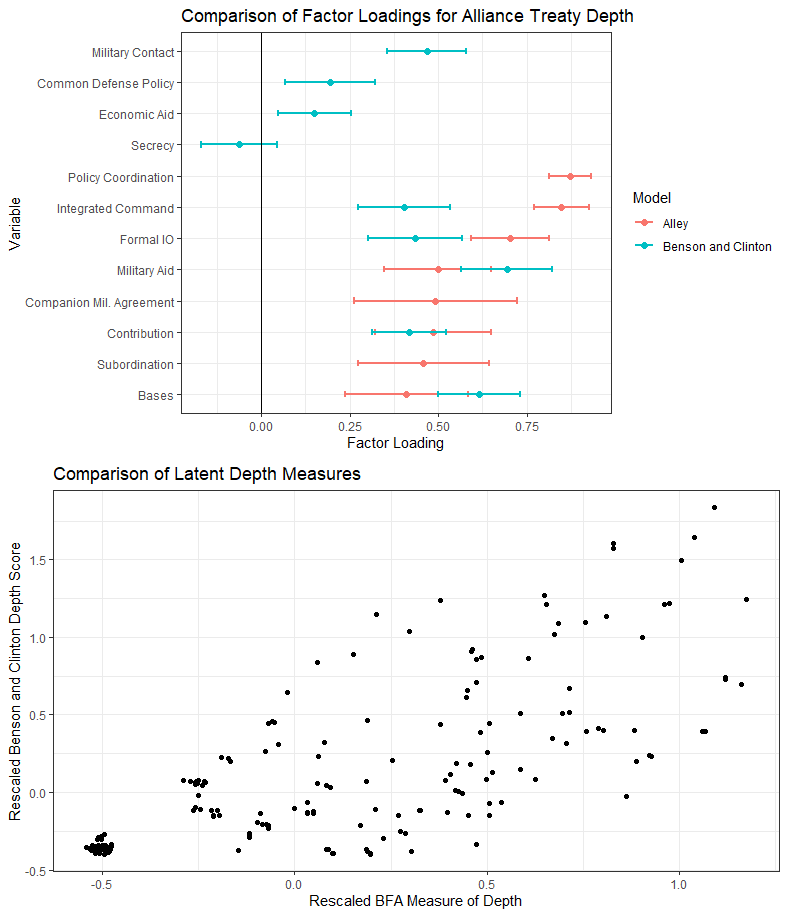
\includegraphics[width=0.95\textwidth]{bc-2016-comp.png}
	\caption{Comparison of latent measures of alliance treaty depth, one from this paper, and the other from \citet{BensonClinton2016}. The top panel compares the factor loadings from the two variables. The scatter plot compares latent depth scores from the semiparametric factor analysis with depth scores from \citet{BensonClinton2016}. The two latent measures have been rescaled by two standard deviations to facilitate comparisons. This comparison only includes alliances for which we both have scores, as I used version 4 of the ATOP data, while Benson and Clinton used version 3.}
	\label{fig:bc-2016-comp}
\end{figure}


In the bottom panel of \autoref{fig:bc-2016-comp}, I plot my measure of treaty depth against Benson and Clinton's. 
To facilitate this comparison, I rescaled both depth measures by dividing them by two standard deviations \citep{Gelman2008}.
Benson and Clinton's measure suggests 5 alliances are well over 3 standard deviations from the mean, while my measure contains no such alliances. 
In general, many treaties Benson and Clinton assign relatively high depth to score somewhat lower relative to other alliances on my measure.
The two measures identify a common set of six extremely deep alliances, however. 
Salient differences in the relative depth of alliance treaties are the result of differences in the factor loadings. 


Though the two measures of depth are correlated, they capture slightly different concepts. 
Benson and Clinton address the general cost of an alliance, while I am focused on military coordination and cooperation. 
Benson and Clinton's measure is useful, but it departs from my aims in this project in important ways. 
Because our measures operationalize different concepts in different subsets of alliances, I believe my measure of depth is better suited for an analysis of deep military cooperation in defensive and offensive alliances. 
My measure is not generally superior and which measure scholars use should depend on how they conceptualize alliance treaty depth. 



  
\bibliography{../../MasterBibliography} 




\end{document}
